\chapter{Figures,tables,enumerate and itemize}

\section{Figures}
graphicx is needed for Figures
    % !h means right here! right here!     [!t] top [!b] bottom
\begin{figure}[!h]
    % center the figure
    \centering
    %   the figure takes 30% of textwidth
    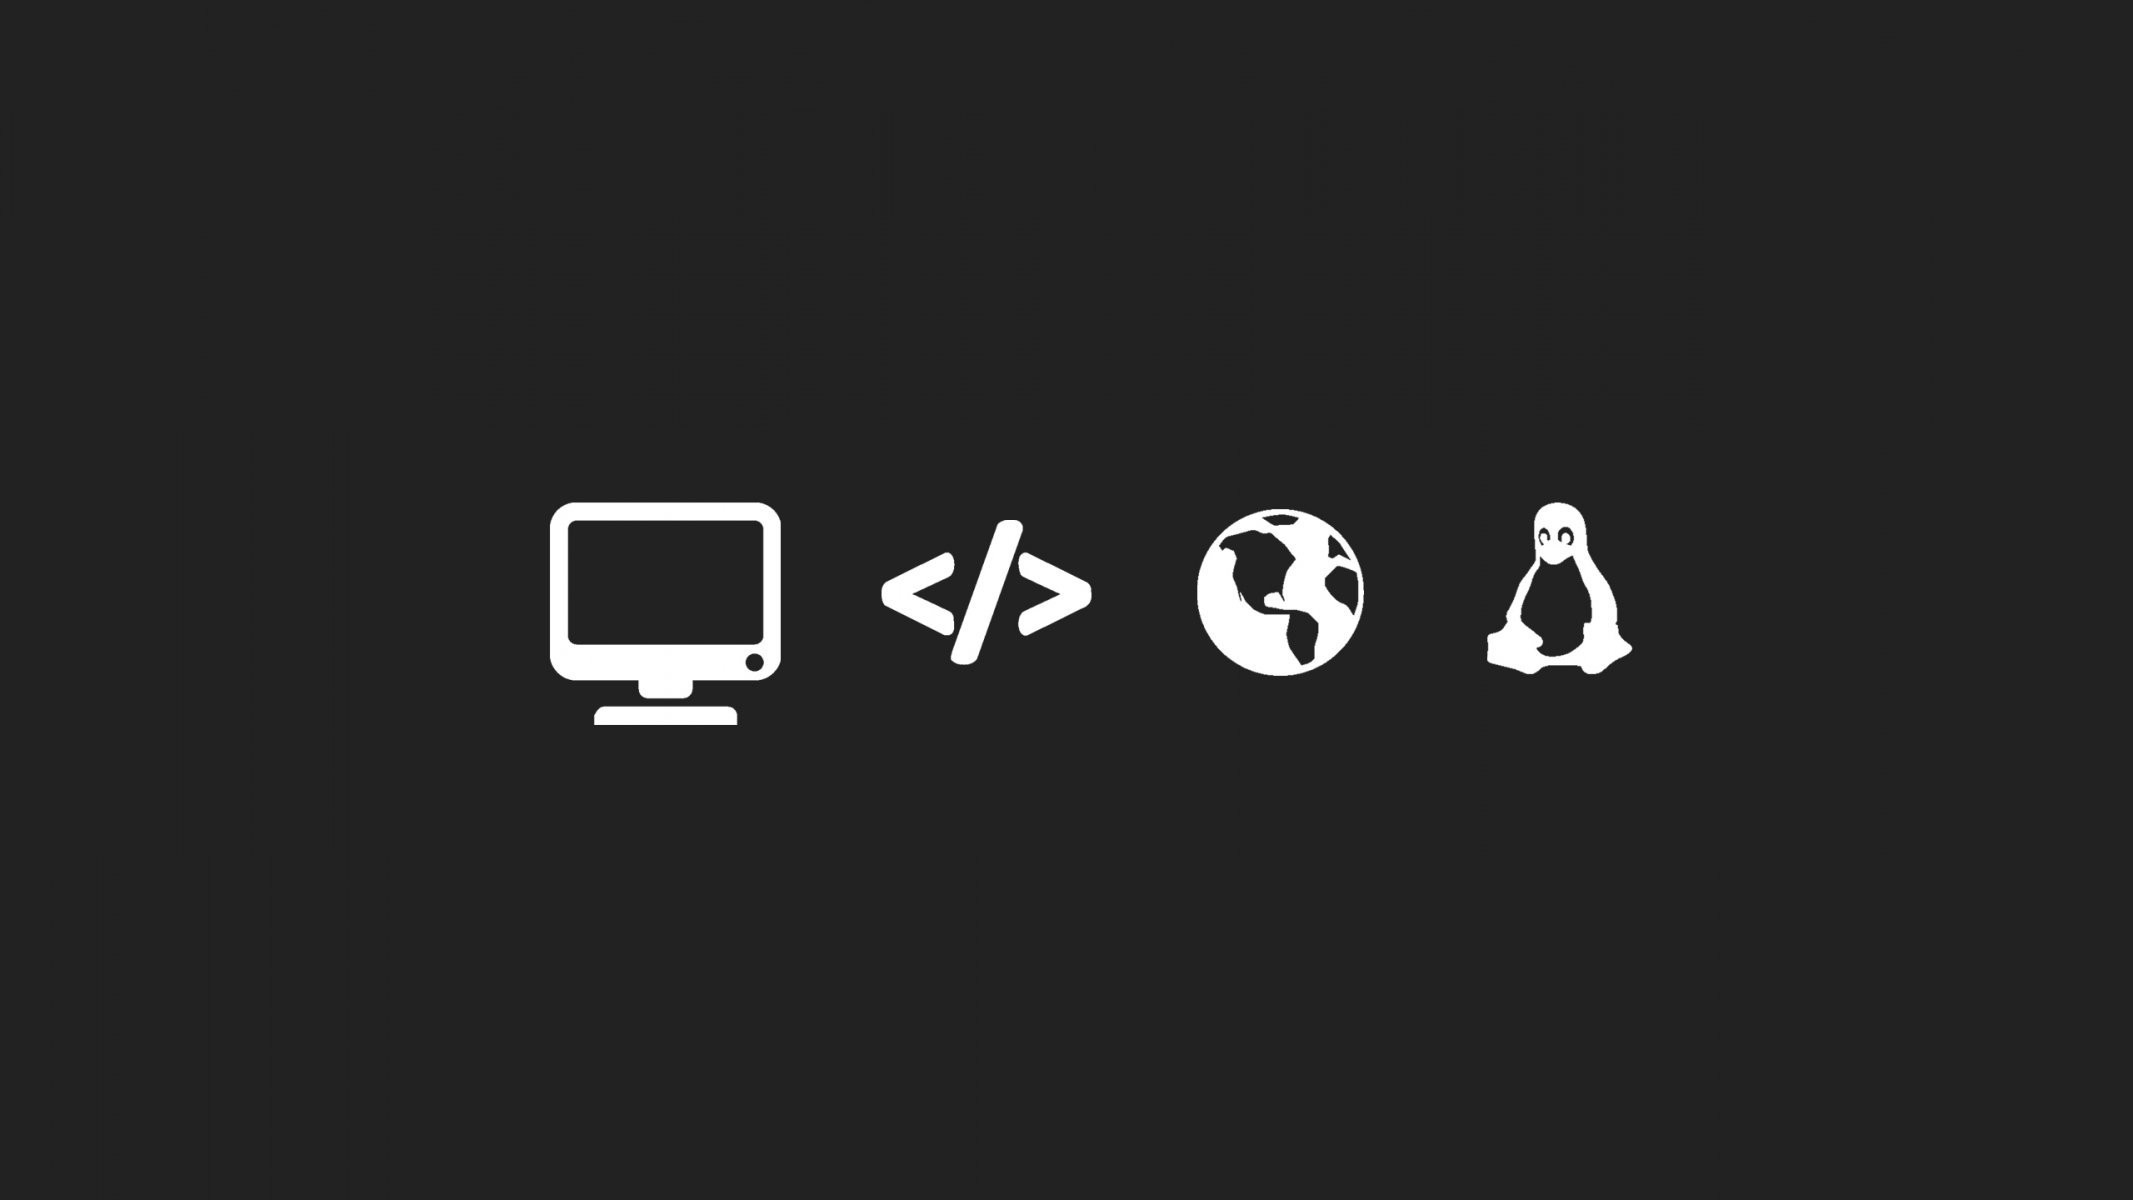
\includegraphics[width=0.3\textwidth]{chapters/chapter2/theWorldIsLinux.jpg}
    \caption{A linux figure}
    \label{linux}
\end{figure}


\newpage

\hyperref[linux]{Linux}

\section{Tables}
Data can be presented in tables,

% no equation environment needed
\begin{table}[!h]
    \centering% a beautiful SQL like table
    \begin{tabular}{l|cl}
        \hline  % horizontal line
        \hline
         & Property 1 & Property 2\\
        \hline
    Car  & Can Run      & Cost gas\\
    Bike & Can Run      & Cost labor\\
        \hline
        \hline
    \end{tabular}
    \caption{Car vs Bike}
    \label{Figure_CarvsBike}
\end{table}

% center make it centered
\begin{center}% like tabular
    \begin{longtable}{l|l|l} % long table can goes to next page and break the page
        \hline  % horizontal line
        \hline

        % define the first head
        & Property 1 & Property 2\\ % the header
        \endfirsthead        % the header will appear on every page
        \hline
        % multicolumn <the number of columns> <left center right> <what to put on the top> 
        
        % define the header
        \multicolumn{3}{c}{\tablename\ \thetable{} -- information message on top}\\
        \hline
        & Property 1 & Property 2\\
        \hline
        \endhead

        % define the foot
        \hline
        \multicolumn{3}{c}{foot information}\\ \hline
        \endfoot

        % define the last foot
        \hline \hline
        \caption{longtable}
        \label{long_table}
        \endlastfoot


        % actual contents of the table

        1 & 2 & 3\\
        1 & 2 & 3\\
        1 & 2 & 3\\
        1 & 2 & 3\\
        1 & 2 & 3\\
        1 & 2 & 3\\
        1 & 2 & 3\\
        1 & 2 & 3\\
        1 & 2 & 3\\
        1 & 2 & 3\\
        1 & 2 & 3\\
        1 & 2 & 3\\
        1 & 2 & 3\\
        1 & 2 & 3\\
        1 & 2 & 3\\
        1 & 2 & 3\\
        1 & 2 & 3\\
        1 & 2 & 3\\
        1 & 2 & 3\\
        1 & 2 & 3\\
        1 & 2 & 3\\
        1 & 2 & 3\\
        1 & 2 & 3\\
        1 & 2 & 3\\
        1 & 2 & 3\\
        1 & 2 & 3\\
        1 & 2 & 3\\
        1 & 2 & 3\\
        1 & 2 & 3\\
        1 & 2 & 3\\
        1 & 2 & 3\\
        1 & 2 & 3\\
        1 & 2 & 3\\
        1 & 2 & 3\\
        1 & 2 & 3\\
        1 & 2 & 3\\
        1 & 2 & 3\\
        1 & 2 & 3\\
        1 & 2 & 3\\
        1 & 2 & 3\\
        1 & 2 & 3\\
        1 & 2 & 3\\
        1 & 2 & 3\\
        1 & 2 & 3\\
        1 & 2 & 3\\
        1 & 2 & 3\\
        1 & 2 & 3\\
        1 & 2 & 3\\
        1 & 2 & 3\\
        1 & 2 & 3\\
        1 & 2 & 3\\
        1 & 2 & 3\\
        1 & 2 & 3\\
        1 & 2 & 3\\
        1 & 2 & 3\\
        1 & 2 & 3
        
    \end{longtable}
\end{center}



\section{Enumerate and itemize}

\begin{enumerate}
\item some stuff
\item more stuff
\end{enumerate}

% use a) b) c)
\begin{enumerate}[a)]
    \item some stuff
    \item more stuff
\end{enumerate}